\documentclass[12pt,a4paper,twoside,openright]{report}
	\usepackage[pdfborder={0 0 0}]{hyperref}    % turns references into hyperlinks
	\usepackage[margin=25mm]{geometry}  % adjusts page layout
	\usepackage{graphicx}  % allows inclusion of PDF, PNG and JPG images
	\usepackage{verbatim}
	\usepackage{docmute}   % only needed to allow inclusion of proposal.tex
	\usepackage{import} %import proposal from another folder
	\usepackage{pdfpages}

	\raggedbottom                           % try to avoid widows and orphans
	\sloppy
	\clubpenalty1000%
	\widowpenalty1000%
	
	\renewcommand{\baselinestretch}{1.1}    % adjust line spacing to make
																					% more readable
	
	\begin{document}
	
	\bibliographystyle{plain}
	
	
	%%%%%%%%%%%%%%%%%%%%%%%%%%%%%%%%%%%%%%%%%%%%%%%%%%%%%%%%%%%%%%%%%%%%%%%%
	% Title
	
	
	\pagestyle{empty}
	
	\rightline{\LARGE \textbf{Charlie Crisp}}
	
	\vspace*{60mm}
	\begin{center}
	\Huge
	\textbf{Building a Blockchain Library for OCaml} \\[5mm]
	Computer Science Tripos -- Part II \\[5mm]
	Pembroke College \\[5mm]
	\today  % today's date
	\end{center}
	
	%%%%%%%%%%%%%%%%%%%%%%%%%%%%%%%%%%%%%%%%%%%%%%%%%%%%%%%%%%%%%%%%%%%%%%%%%%%%%%
	% Proforma, table of contents and list of figures
	
	\pagestyle{plain}
	
	\chapter*{Proforma}
	
	{\large
	\begin{tabular}{ll}
	Name:               & \bf Charlie Crisp                       \\
	College:            & \bf Pembroke College                     \\
	Project Title:      & \bf Building a Blockchain Library for OCaml \\
	Examination:        & \bf Computer Science Tripos -- Part II, July 2018  \\
	Word Count:         & \bf ????\footnotemark[1]
												(well less than the 12000 limit)  \\
	Project Originator: & KC Sivaramakrishnan                    \\
	Supervisor:         & KC Sivaramakrishnan                    \\ 
	\end{tabular}
	}
	\footnotetext[1]{This word count was computed
	by \texttt{detex diss.tex | tr -cd '0-9A-Za-z $\tt\backslash$n' | wc -w}
	}
	\stepcounter{footnote}
	
	
	\section*{Original Aims of the Project}
	
	To build a library in OCaml, which can be used as a building block for Blockchain applications. 
	The library should allow participating nodes to own a shared copy of a Blockchain data structure, agreed upon using consensus.
	Nodes should also be able to commit transactions to the blockchain, which should then be visible to other participating nodes. 
	
	
	\section*{Work Completed}
	
	All that has been completed appears in this dissertation.
	
	\section*{Special Difficulties}
	
	None
	 
	\newpage
	\section*{Declaration}
	
	I, Charlie Crisp of Pembroke College, being a candidate for Part II of the Computer
	Science Tripos [or the Diploma in Computer Science], hereby declare
	that this dissertation and the work described in it are my own work,
	unaided except as may be specified below, and that the dissertation
	does not contain material that has already been used to any substantial
	extent for a comparable purpose.
	
	\bigskip
	\leftline{Signed [signature]}
	
	\medskip
	\leftline{Date [date]}
	
	\tableofcontents
	
	\listoffigures
	
	\newpage
	\section*{Acknowledgements}
	
	I would like to thank KC Sivaramakrishnan for being an extremely helpful supervisor throughout the duration of the dissertation, as well as over the past three years.\\
	I would also like to thank Anil Madhavapeddy for allowing me to use his laptop for the duration of the dissertation, and being a very supportive DoS.\\
	Finally I'd like to thank my friends and family for supporting me through my final year.
	
	%%%%%%%%%%%%%%%%%%%%%%%%%%%%%%%%%%%%%%%%%%%%%%%%%%%%%%%%%%%%%%%%%%%%%%%
	% now for the chapters
	
	\pagestyle{headings}
	
	\chapter{Introduction}
	
	The lecture suggests putting a paragraph here to explain the project, and how well it's been completed. Question - how is this different to what is on page 3?

	\section{What is the Blockchain?}
	
	The blockchain, in its simplest form, is a series of blocks of data, where each block contains the cryptographic hash of the previous block in the chain. This means that the chain can exhibit arbitrary branching. Figure \ref{fig:mainblockchain} is a graphical representation of a typical blockchain data structure.\\
	The significance of blocks containing hashes of previous blocks, is that if a change were to be made to a previous block, it would change the hashes of all subsequent blocks in the chain. This means that once a block is committed to the blockchain, it cannot be modified. \\
	\\
	\begin{figure}
		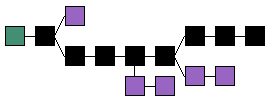
\includegraphics[width=\linewidth]{figs/blockchain}
		\caption{A typical blockchain structure}
		\label{fig:mainblockchain}
	\end{figure}
	
	\section{The History of the Blockchain}
	The blockchain, as a cryptographically secure chain of blocks, was first conceptualised by Stuart Haber and W. Scott Stornetta in 1990 \cite{HaberStornetta}.
	However, until the creation of Git \cite{Git} in 2005, the blockchain was still a relatively niche concept.\\
	Git uses the blockchain as a basis for storing a secure history of code in the form of commits made to branches.
	We will explore the use of the Git as a blockchain during chapter ??? \\
	\\
	The invention of Bitcoin\cite{Bitcoin} in 2008 is seen by many as the most pivotal moment in the history of blockchain technologies.
	Bitcoin combines the blockchain with a 'Proof of Work' consensus algorithm and the result of this is a decentralised, trust-less, peer to peer network which doesn't suffer from the double spending problem. \\
	\\
	\section{Blockchain Today}
	At the time of writing, cryptocurrencies are generating a huge amount of excitement and cynicism in technology and economics communities. The value of Bitcoin is fluctuating on a day-by-day basis and many alternative currencies are gaining in popularity.\\
	For example, Ethereum is a blockchain platform that allows participants to run arbitrary\footnote{Whilst there are restrictions to code run on the blockchain (e.g. it has to be deterministic), the Ethereum language is Turing complete.} code on the blockchain. This is known as Smart Contracts.

	\chapter{Preparation}
	Things to mention:\\
		Consensus algorithms:\\
		Proof of work\\
		Proof of stake\\
		Paxos\\
		Raft\\
	Irmin and Ezirmin\\
		Git as a blockchain\\
			with hashing and branching and all\\
			\\
	Other blockchain architecture including mempools\\
	\\
	Requirements analysis
	
	\chapter{Implementation}
	
	\chapter{Evaluation}
	
	\chapter{Conclusion}
	
	
	%%%%%%%%%%%%%%%%%%%%%%%%%%%%%%%%%%%%%%%%%%%%%%%%%%%%%%%%%%%%%%%%%%%%%
	% the bibliography
	\bibliographystyle{plain}
	\bibliography{refs}
	\addcontentsline{toc}{chapter}{Bibliography}
	
	%%%%%%%%%%%%%%%%%%%%%%%%%%%%%%%%%%%%%%%%%%%%%%%%%%%%%%%%%%%%%%%%%%%%%
	% the appendices
	\appendix

	\chapter{Project Proposal}
	
	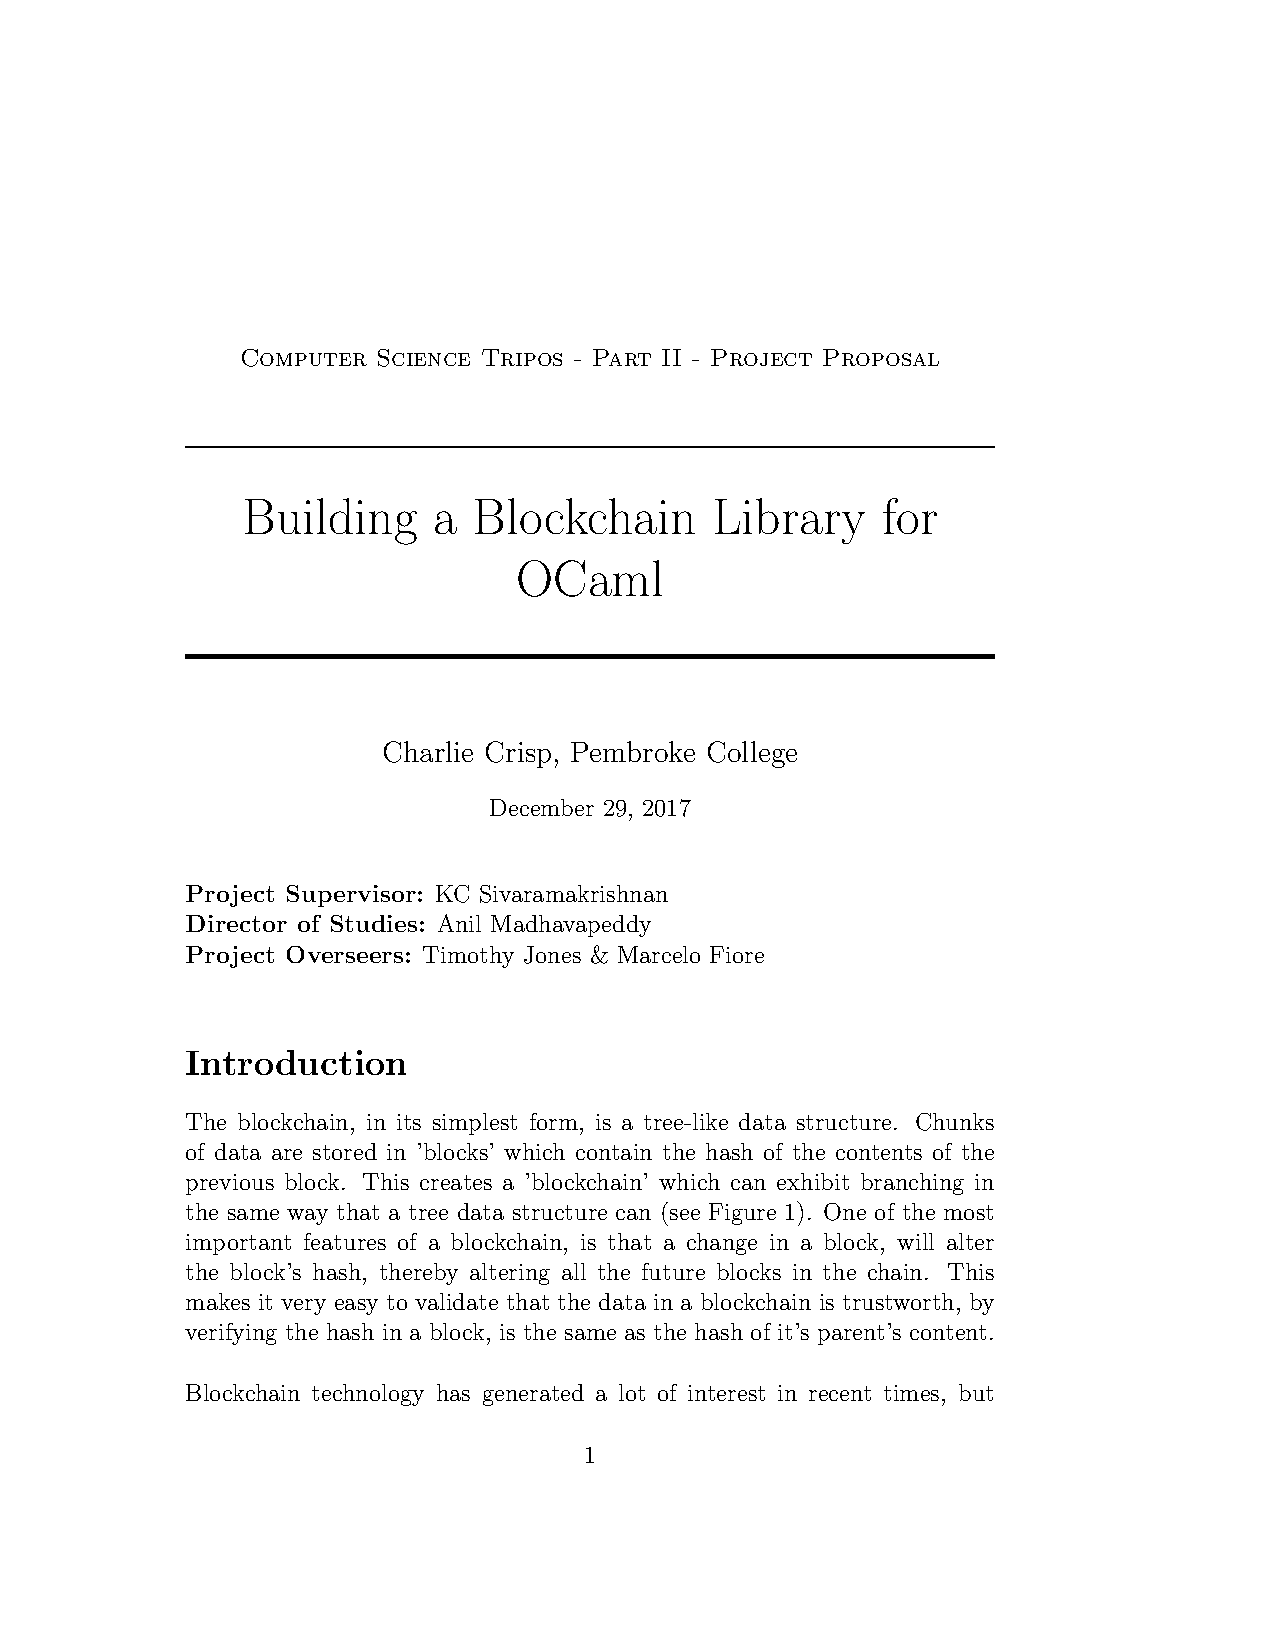
\includepdf[pages=-]{Part_II_Project_Proposal_Draft.pdf}
	
	\end{document}